\documentclass{minimal}

\usepackage{lmodern}

\usepackage{tikz}
\usepackage{xspace}
\usepackage{makecell}
\usepackage{amsmath}

\newcommand{\acl}{\textsf{LSE}\xspace}

\usetikzlibrary{arrows,positioning,shapes,fit}
\tikzset{
    %Define standard arrow tip
    >=stealth',
    %Define style for boxes
    st/.style={
           rectangle,
           %rounded corners,
           draw=black, very thick,
           %text width=6.5em,
           minimum height=2em,
           text centered},
    % Define arrow style
    pil/.style={
           ->,
           thick,
           shorten <=2pt,
           shorten >=2pt,}
}

\definecolor{col1}{RGB}{140,191,38}

\begin{document}
\hspace{-8em}
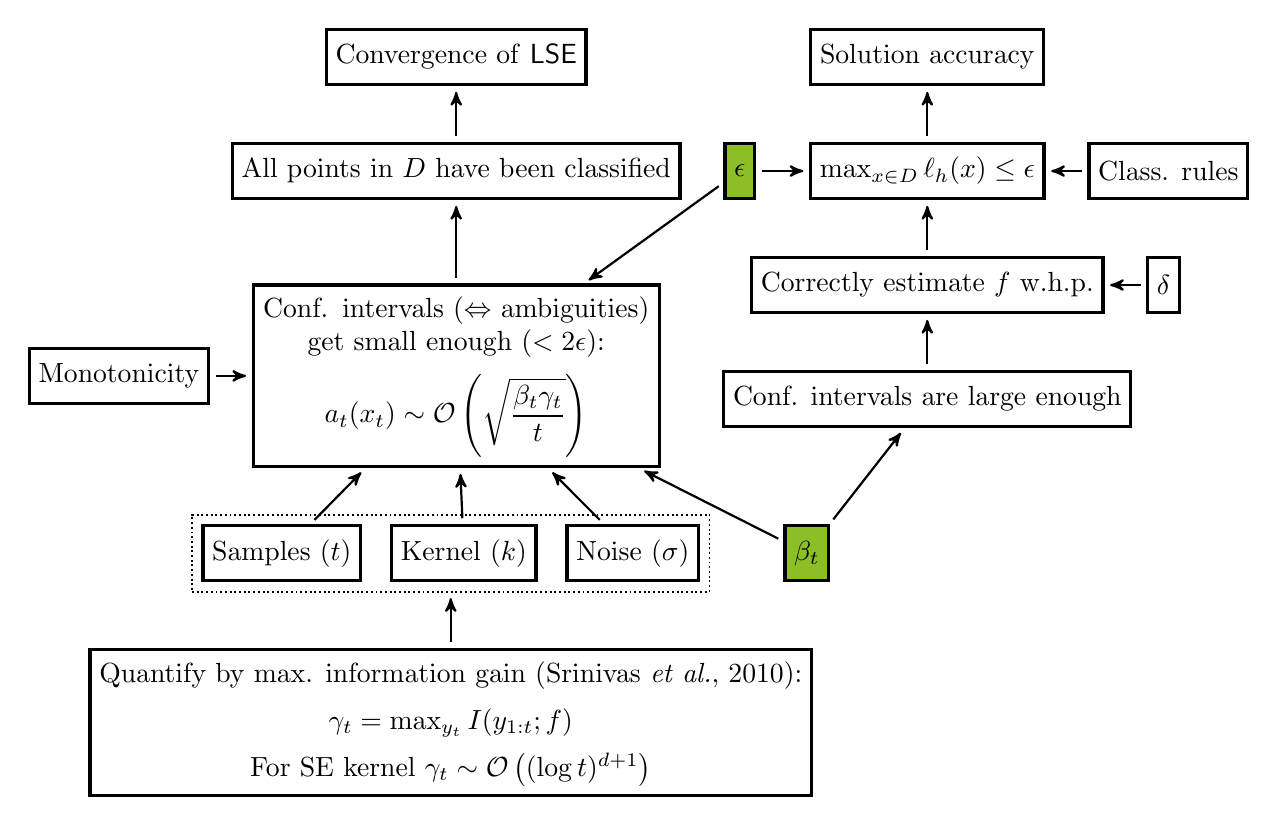
\begin{tikzpicture}[node distance=1cm, auto,]
 %nodes
 \node[st] (conv) {Convergence of \acl};
   
 \node[st,below=2em of conv] (clas) {All points in $D$ have been classified}
   edge[pil] (conv);

 \node[st,text width=14em,below=3em of clas] (amb)
 {\makecell[c]
   {Conf. intervals ($\Leftrightarrow$ ambiguities)\\
    get small enough ($<2\epsilon$):\\[0.5em]
    $a_t(\*x_t) \sim \mathcal{O}\left(\sqrt{\displaystyle\frac{\beta_t\gamma_t}{t}}\right)$
   }
 } edge[pil] (clas);
 
 \node[st,draw=none,below=2em of amb] (dummy) {};

 \node[st,left=1.5em of amb] (t0) {Monotonicity}
   edge[pil] (amb);
 \node[st,left=3em of dummy] (t1) {Samples ($t$)}
   edge[pil] (amb);
 \node[st,right=1em of t1] (t2) {Kernel ($k$)}
   edge[pil] (amb);
 \node[st,right=1em of t2] (t3) {Noise ($\sigma$)}
   edge[pil] (amb);
 \node[st,right=3em of t3,fill=col1] (t4) {$\beta_t$}
   edge[pil] (amb);
   
 \node[draw=black,densely dotted,line width=0.7pt,fit=(t1)(t3)] (fit1) {};
 
 \node[st,below=2em of fit1] (gamma)
 {\makecell[c]
   {Quantify by max. information gain (Srinivas \emph{et al.}, 2010):\\[0.5em]
    $\gamma_t = \max_{\*y_t} I(\*y_{1:t}; f)$\\[0.5em]
    For SE kernel $\gamma_t \sim \mathcal{O}\left((\log t)^{d+1}\right)$
   }
 } edge[pil] (fit1);
 
 \node[st,right=8em of conv] (acc) {Solution accuracy};
 
 \node[st,below=2em of acc] (loss) {$\max_{\*x\in D} \ell_h(\*x) \leq \epsilon$}
   edge[pil] (acc);
 
 \node[st,right=1.5em of loss] (rules) {Class. rules}
   edge[pil] (loss);
   
 \node[st,below=2em of loss] (est) {Correctly estimate $f$ w.h.p.}
   edge[pil] (loss);
   
 \node[st,right=1.5em of est] (delta) {$\delta$}
   edge[pil] (est);
   
 \node[st,below=2em of est] (large) {Conf. intervals are large enough}
   edge[pil] (est)
   edge[pil,<-] (t4);
   
 \node[st,right=1.5em of clas,fill=col1] (eps) {$\epsilon$}
   edge[pil] (amb)
   edge[pil] (loss);
\end{tikzpicture}
\end{document}
